% Numbers below are copied from results/summary/*.md (generated by scripts/aggregate.py);
% the tables are generated by scripts/make_tables.py.
\begin{table*}[!t]
\centering
\caption{Results at a 250,000-event budget: mean$\pm$sd over 5 seeds, all scored on the same 500k test events. ECE before and after post-hoc calibration on the cal split. Bold: best ROC AUC within the feature set.}
\label{tab:ml_main}
\footnotesize
\setlength{\tabcolsep}{3.5pt}
\begin{tabular}{lcccccccc}
\toprule
Features & Model & ROC AUC & PR AUC & Brier & ECE & ECE$_\mathrm{Platt}$ & ECE$_\mathrm{iso}$ & Train s \\
\midrule
low (21) & LogReg & 0.5957$\pm$0.0001 & 0.6224$\pm$0.0002 & 0.2418$\pm$0.0000 & 0.0155 & 0.0157 & 0.0054 & 0.1 \\
low (21) & XGBoost & \textbf{0.7376$\pm$0.0006} & 0.7481$\pm$0.0006 & 0.2064$\pm$0.0002 & 0.0053 & 0.0058 & 0.0072 & 5.1 \\
geo (40) & LogReg & 0.6298$\pm$0.0001 & 0.6494$\pm$0.0003 & 0.2357$\pm$0.0000 & 0.0079 & 0.0084 & 0.0053 & 0.1 \\
geo (40) & XGBoost & \textbf{0.8011$\pm$0.0005} & 0.8111$\pm$0.0005 & 0.1812$\pm$0.0002 & 0.0037 & 0.0034 & 0.0081 & 11.6 \\
high (7) & LogReg & 0.6450$\pm$0.0004 & 0.6168$\pm$0.0006 & 0.2322$\pm$0.0000 & 0.0480 & 0.0483 & 0.0061 & 0.0 \\
high (7) & XGBoost & \textbf{0.7872$\pm$0.0003} & 0.8050$\pm$0.0003 & 0.1872$\pm$0.0001 & 0.0062 & 0.0051 & 0.0065 & 1.5 \\
all (28) & LogReg & 0.6842$\pm$0.0002 & 0.6828$\pm$0.0003 & 0.2231$\pm$0.0000 & 0.0242 & 0.0246 & 0.0061 & 0.1 \\
all (28) & XGBoost & \textbf{0.8235$\pm$0.0006} & 0.8378$\pm$0.0005 & 0.1711$\pm$0.0003 & 0.0053 & 0.0061 & 0.0067 & 4.8 \\
geo+high (47) & LogReg & 0.6918$\pm$0.0002 & 0.6924$\pm$0.0002 & 0.2206$\pm$0.0000 & 0.0181 & 0.0185 & 0.0064 & 0.2 \\
geo+high (47) & XGBoost & \textbf{0.8381$\pm$0.0003} & 0.8506$\pm$0.0004 & 0.1638$\pm$0.0001 & 0.0054 & 0.0053 & 0.0078 & 10.4 \\
\bottomrule
\end{tabular}
\end{table*}


\subsection{Fixed budget: 250k events, five seeds}
Table~\ref{tab:ml_main} reports every metric as mean$\pm$sd over five seeds. The seed-to-seed sd of
the ROC AUC never exceeds 0.0007, and every difference cited below is significant under the paired
DeLong test in all five seeds ($p<10^{-6}$; Table~\ref{tab:comparisons}).

\begin{table*}[!t]
\centering
\caption{Paired DeLong tests on the shared test set. $\Delta$AUC = A$-$B (mean$\pm$sd over seeds); last column: seeds in which the difference is significant at $\alpha=0.05$ in favour of A / B.}
\label{tab:comparisons}
\footnotesize
\setlength{\tabcolsep}{3.5pt}
\begin{tabular}{lllcc}
\toprule
Question & A & B & $\Delta$AUC & Sig. A/B \\
\midrule
DL vs trees on raw measurements & mlp|low & xgboost|low & 0.0226$\pm$0.0011 & 5/0 \\
DL vs trees on geometric features & mlp|geo & xgboost|geo & 0.0244$\pm$0.0006 & 5/0 \\
DL vs trees on raw + expert & mlp|all & xgboost|all & 0.0075$\pm$0.0005 & 5/0 \\
Feature engineering (geo) for trees & xgboost|geo & xgboost|low & 0.0635$\pm$0.0008 & 5/0 \\
Feature engineering (geo) for the MLP & mlp|geo & mlp|low & 0.0654$\pm$0.0010 & 5/0 \\
Geometry alone vs expert masses (MLP) & mlp|geo & mlp|high & 0.0325$\pm$0.0011 & 5/0 \\
Geometry alone vs expert masses (XGB) & xgboost|geo & xgboost|high & 0.0139$\pm$0.0004 & 5/0 \\
Geometry alone vs raw + expert (MLP) & mlp|geo & mlp|all & -0.0055$\pm$0.0011 & 0/5 \\
geo+expert vs raw+expert (MLP) & mlp|geo\_high & mlp|all & 0.0112$\pm$0.0012 & 5/0 \\
Hybrid 1: wide\&deep vs plain MLP, same inputs & widedeep|geo\_high & mlp|geo\_high & -0.0092$\pm$0.0008 & 0/5 \\
Hybrid 2: stacking vs MLP & stack|geo\_high & mlp|geo\_high & 0.0084$\pm$0.0008 & 5/0 \\
Hybrid 2: stacking vs XGB & stack|geo\_high & xgboost|geo\_high & 0.0124$\pm$0.0001 & 5/0 \\
Hybrid 2: learned stacking vs naive average & stack|geo\_high & average|geo\_high & 0.0002$\pm$0.0000 & 5/0 \\
Hybrid 2 on the paper's features: stacking vs MLP & stack|all & mlp|all & 0.0044$\pm$0.0005 & 5/0 \\
\bottomrule
\end{tabular}
\end{table*}


\textbf{RQ1, value of the expert features.} Logistic regression is close to useless on the raw
measurements (AUC 0.596). The 7 masses lift it to 0.645, and \texttt{all} to 0.684. XGBoost reaches
0.738 on \texttt{low} and 0.787 on \texttt{high}. Combining raw and expert features (\texttt{all},
0.823) adds a further 0.036 over the masses alone. The expert features are therefore worth roughly
0.05--0.09 AUC to both models. Even so, the trees extract substantial information that the masses
do not contain.

\textbf{RQ2, symmetry-derived features.} Replacing the five absolute angles with pairwise
$|\Delta\phi|$ and $\Delta R$ (\texttt{geo}, no masses) raises XGBoost from 0.738 to 0.801
($\Delta=+0.064$). It also lets XGBoost \emph{beat the expert masses} ($+0.014$ over \texttt{high}).
Logistic regression gains $+0.034$ from the same change. Adding the masses to the geometric
features (\texttt{geo+high}) gives the best ML model, XGBoost at 0.838. That is $+0.015$ over the
paper's \texttt{all} feature set. Physical symmetry, with no reconstruction of intermediate
particles, recovers most of what the expert features provide, and it complements them.

\textbf{RQ3, calibration.} XGBoost is well calibrated out of the box (ECE 0.004--0.006), and Platt
scaling leaves it unchanged. Logistic regression shows the opposite failure. Its probabilities are
miscalibrated precisely where the model is misspecified: ECE 0.048 on \texttt{high}, whose masses
relate to the label non-monotonically (Fig.~\ref{fig:shapdep}). Platt scaling cannot fix this
(0.048), because a monotone affine map of the logit cannot change the curve's shape. Isotonic
regression reduces it to 0.006. Fig.~\ref{fig:reliability} shows the reliability diagrams.

\begin{figure*}[!t]
\centering
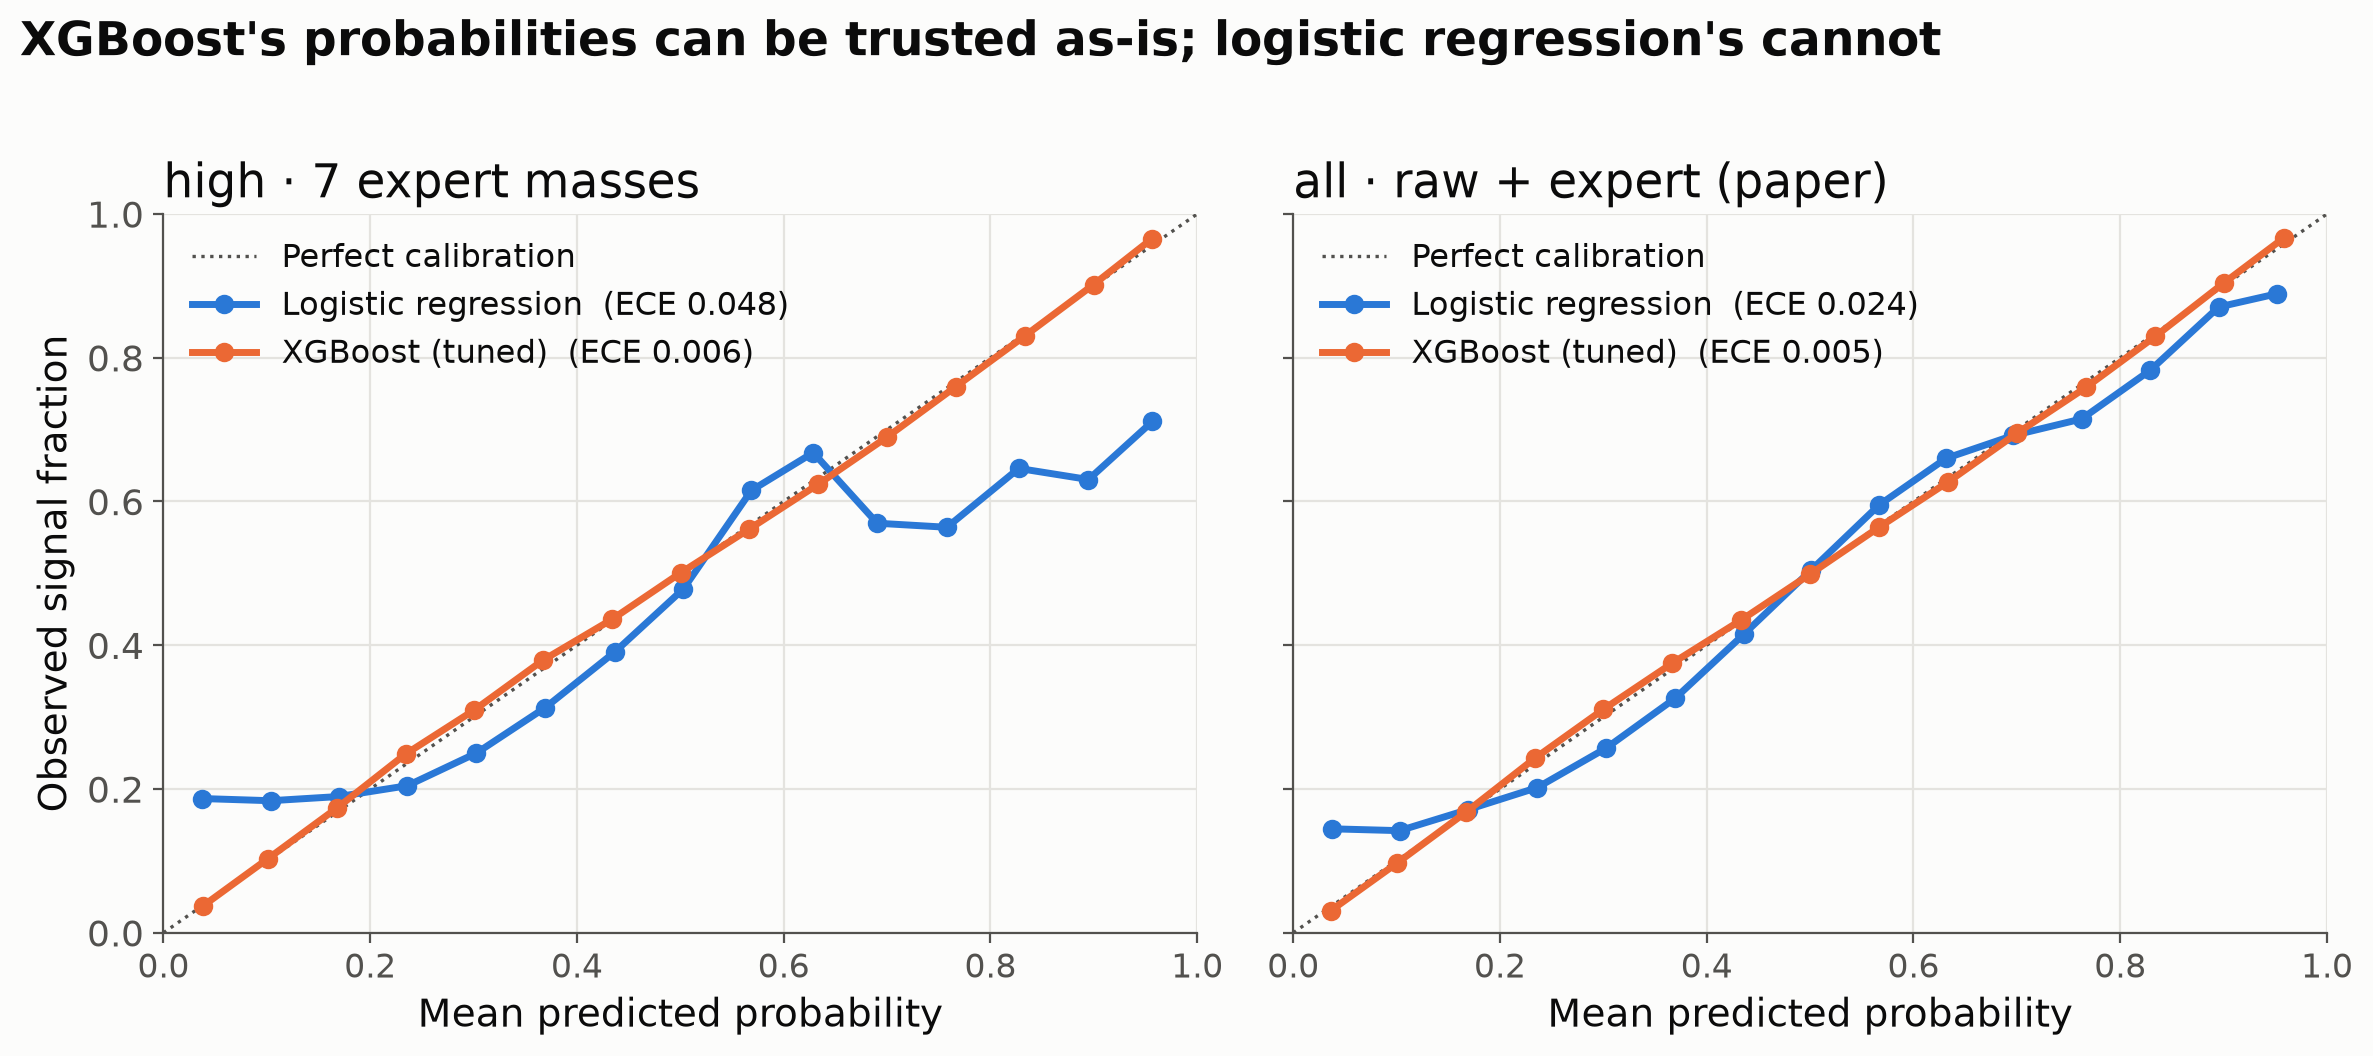
\includegraphics[width=0.85\textwidth]{reliability_ml.png}
\caption{Reliability diagrams on the 500k test events (seed~0, 250k budget, before post-hoc
calibration), for the 7 expert masses (left) and the paper's 28 features (right). XGBoost (orange)
follows the diagonal; logistic regression (blue) bends wherever its linear log-odds are misspecified.}
\label{fig:reliability}
\end{figure*}

\textbf{Compute.} At 250k events, logistic regression trains in under 0.2\,s. Tuned XGBoost needs
1.5\,s (\texttt{high}, 7 features) to 11.6\,s (\texttt{geo}, 40 features, depth 10). The cheapest
strong model is XGBoost on \texttt{all} (4.8\,s, AUC 0.823).

\subsection{Tuning}
Table~\ref{tab:tuning} shows that CV favours deep trees (depth 10 on \texttt{low}/\texttt{geo}, 8
otherwise), a learning rate of 0.05 and a large \texttt{min\_child\_weight} (20). Deep trees are
consistent with the target being a high-order interaction of the raw inputs. Tuning improved
XGBoost by 0.004--0.015 AUC over our initial defaults. For logistic regression the CV AUC varies by
less than $10^{-3}$ across $C$, so the edge-of-grid choices are immaterial.

\subsection{Interpretability}
\begin{table}[!t]
\centering
\caption{Top-10 features of the \texttt{all} set by XGBoost mean $|$SHAP$|$ (log-odds), with logistic-regression $|$coefficients$|$ on standardised inputs.}
\label{tab:importance_ml}
\footnotesize
\setlength{\tabcolsep}{3.5pt}
\begin{tabular}{lcc}
\toprule
Feature & XGB $|$SHAP$|$ & LogReg $|\beta|$ \\
\midrule
m\_bb & 0.635 & 0.600 \\
m\_wwbb & 0.514 & 0.996 \\
m\_wbb & 0.340 & 0.624 \\
m\_jjj & 0.317 & 0.265 \\
m\_jlv & 0.276 & 0.204 \\
jet1\_pt & 0.258 & 0.365 \\
lepton\_pT & 0.172 & 0.171 \\
missing\_energy\_magnitude & 0.134 & 0.238 \\
m\_jj & 0.129 & 0.098 \\
jet2\_pt & 0.102 & 0.087 \\
\bottomrule
\end{tabular}
\end{table}

Both models rank the masses first (Table~\ref{tab:importance_ml}), led by $m_{bb}$ for XGBoost and
$m_{WWbb}$ for logistic regression. The SHAP dependence plots (Fig.~\ref{fig:shapdep}) recover the
physics without being told it. Events whose $m_{bb}$ falls in the peak where $h^0\!\to b\bar b$
decays land are pushed towards signal, by up to $+1$ in log-odds. Events whose three-jet mass
$m_{jjj}$ lies near the top-quark peak are pushed towards \emph{background}, the
$t\!\to\!Wb\!\to\!jjb$ signature. On \texttt{geo}, without masses, XGBoost relies on jet and lepton
$p_T$, the $b$-tags, $|E_T^\mathrm{miss}|$ and the lepton--jet $\Delta R$ values. Those are the
ingredients from which the masses are built.

\begin{figure*}[!t]
\centering
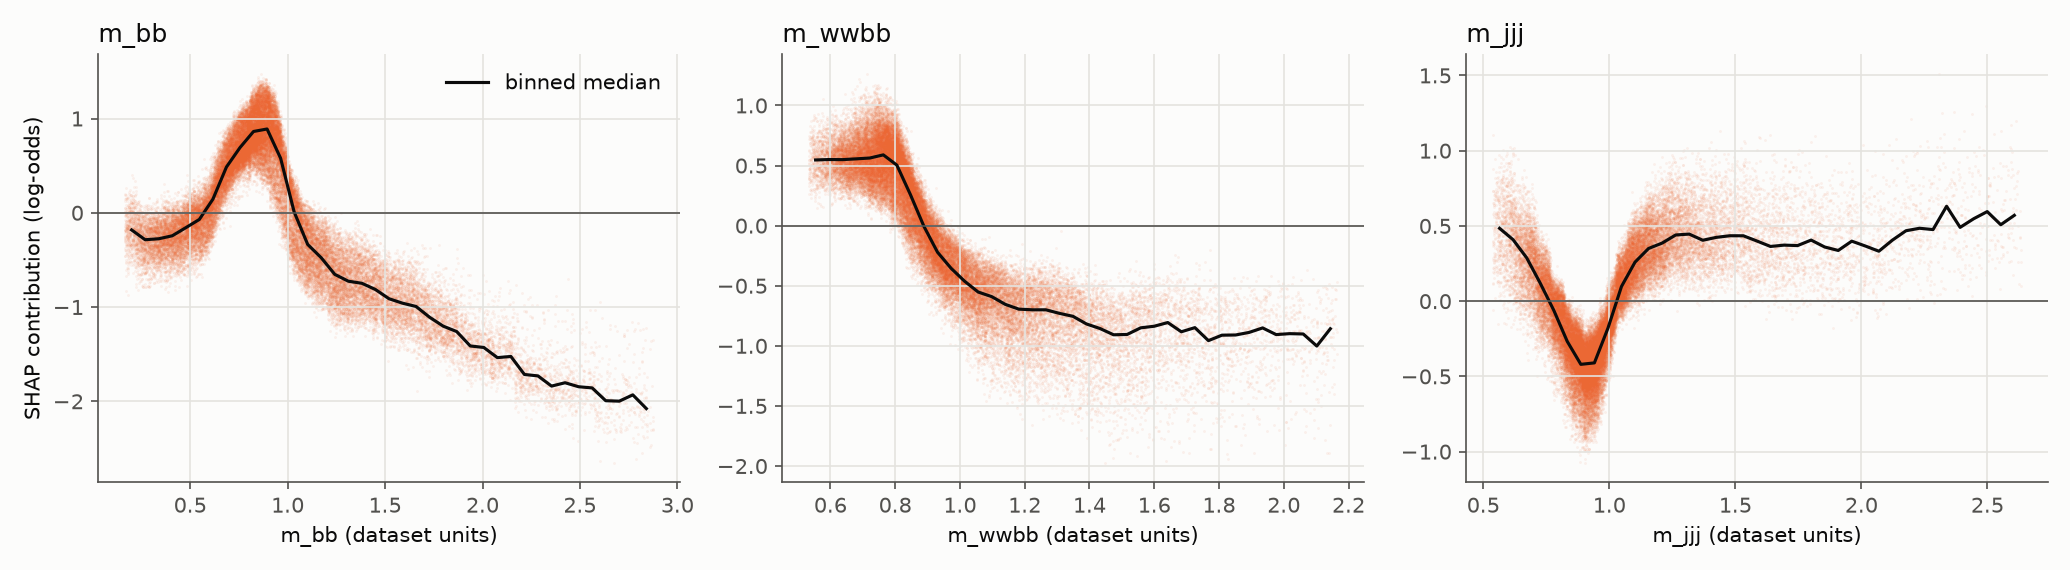
\includegraphics[width=0.92\textwidth]{shap_dependence.png}
\caption{XGBoost TreeSHAP dependence on 50k test events (\texttt{all}, seed~0). Positive values push
towards signal. The $m_{bb}$ peak ($h^0\!\to b\bar b$) favours signal, and the $m_{jjj}$ peak at
the top-quark mass favours the $t\bar t$ background.}
\label{fig:shapdep}
\end{figure*}

\subsection{Scaling beyond the fixed budget}
\begin{table*}[!t]
\centering
\caption{Test ROC AUC vs data budget (train+val+cal events); mean$\pm$sd over seeds (3 seeds; 5 at 250k; 1 at 10.5M, \texttt{low}/\texttt{all} only).}
\label{tab:scaling_ml}
\footnotesize
\setlength{\tabcolsep}{3.5pt}
\begin{tabular}{lccccc}
\toprule
Features & Model & 50k & 250k & 1M & 10.5M \\
\midrule
low (21) & LogReg & 0.5945$\pm$0.0003 & 0.5957$\pm$0.0001 & 0.5959$\pm$0.0000 & 0.5959 \\
low (21) & XGBoost & 0.6986$\pm$0.0011 & 0.7376$\pm$0.0006 & 0.7648$\pm$0.0012 & 0.8001 \\
geo (40) & LogReg & 0.6287$\pm$0.0004 & 0.6298$\pm$0.0001 & 0.6298$\pm$0.0001 & -- \\
geo (40) & XGBoost & 0.7618$\pm$0.0018 & 0.8011$\pm$0.0005 & 0.8230$\pm$0.0005 & -- \\
high (7) & LogReg & 0.6442$\pm$0.0017 & 0.6450$\pm$0.0004 & 0.6450$\pm$0.0003 & -- \\
high (7) & XGBoost & 0.7791$\pm$0.0007 & 0.7872$\pm$0.0003 & 0.7918$\pm$0.0002 & -- \\
all (28) & LogReg & 0.6835$\pm$0.0006 & 0.6842$\pm$0.0002 & 0.6842$\pm$0.0001 & 0.6844 \\
all (28) & XGBoost & 0.8073$\pm$0.0007 & 0.8235$\pm$0.0006 & 0.8365$\pm$0.0001 & 0.8507 \\
geo+high (47) & LogReg & 0.6908$\pm$0.0003 & 0.6918$\pm$0.0002 & 0.6918$\pm$0.0001 & -- \\
geo+high (47) & XGBoost & 0.8180$\pm$0.0005 & 0.8381$\pm$0.0003 & 0.8528$\pm$0.0003 & -- \\
\bottomrule
\end{tabular}
\end{table*}

Table~\ref{tab:scaling_ml} repeats the study at 50k, 1M and the full 10.5M pool. Logistic
regression is flat to within $10^{-3}$ from 50k to 10.5M. It is bias-limited: more data cannot fix a
linear decision boundary. XGBoost keeps improving on every representation, with the largest gains on
raw inputs (\texttt{low}: $0.699\to0.800$). The improvement on the 7 masses saturates quickly
($0.779\to0.792$ from 50k to 1M). At full scale XGBoost reaches 0.851 on \texttt{all}, with the
caveat in Section~\ref{sec:discussion}.
